\chapter{Theoretischer Teil} \label{theorie}

\section{Einleitung} \label{theorieeinleitung}


\section{Messverfahren} \label{messverfahren}
Das Spektrometer misst die Werte immer im gleichen Verfahren. Als R�ckgabe vom Ger�t wird immer die gleiche Datenstruktur verarbeitet. Diese ist unter genauer beschrieben. Damit sp�ter die drei Verfahren angewendet und in Dateien abgespeichert werden k�nnen m�ssen einige Referenz-Werte vorg�ngig vorhanden sein. Diese Werden zum Teil ebenfalls direkt mit dem Spektrometer erfasst, wie eine White Reference oder Dark Current. Referenz-Werte f�r die Radiance-Berechnung sprich die Base, Lamp und FiberOptic Datei werden beim Konfigurieren des Spektrometers in die App importiert und abgespeichert.

\subsection{Abspeichern vs. Anzeigen}
Die berechneten Daten der Reflectance und Radiance werden in der App nur angezeigt aber niemals in eine Datei geschrieben. Die Daten die in den Messdateien abgespeichert werden sind immer Raw Daten. In den Messdateien sind somit alle Daten vorhanden um sp�ter wieder eine Reflectance oder Radiance Berechnung durchzuf�hren.

\begin{figure}[h]
	\begin{center}
		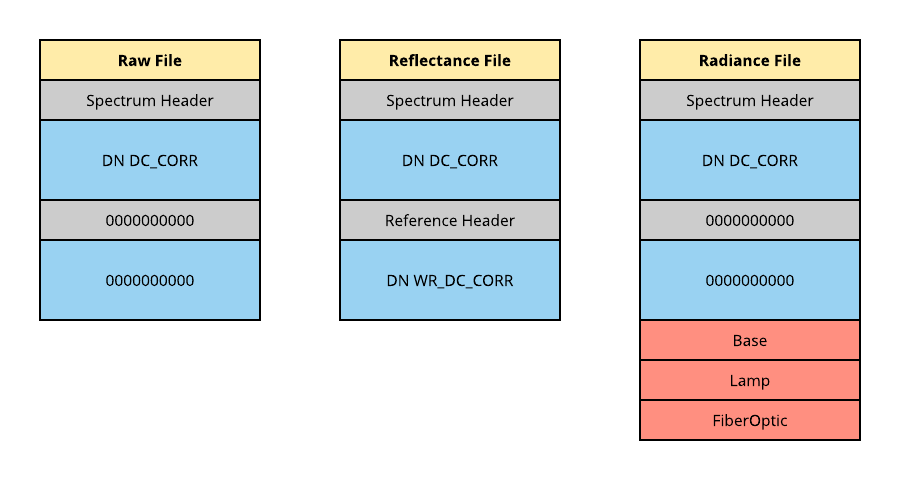
\includegraphics[scale=0.35]{images/IndicoFileFormats} 
	\caption{Berechnungen f�r Raw, Reflectance und Radiance}
	\label{fig:MeasurementFiles}
	\end{center}
\end{figure}



\section{Berechnungsablauf} \label{berechnungsablauf}
Der Berechnungsablauf der drei im App einstellbaren Messverfahren wird am besten in einem Diagramm ersichtlich.

\begin{figure}[h]
	\begin{center}
		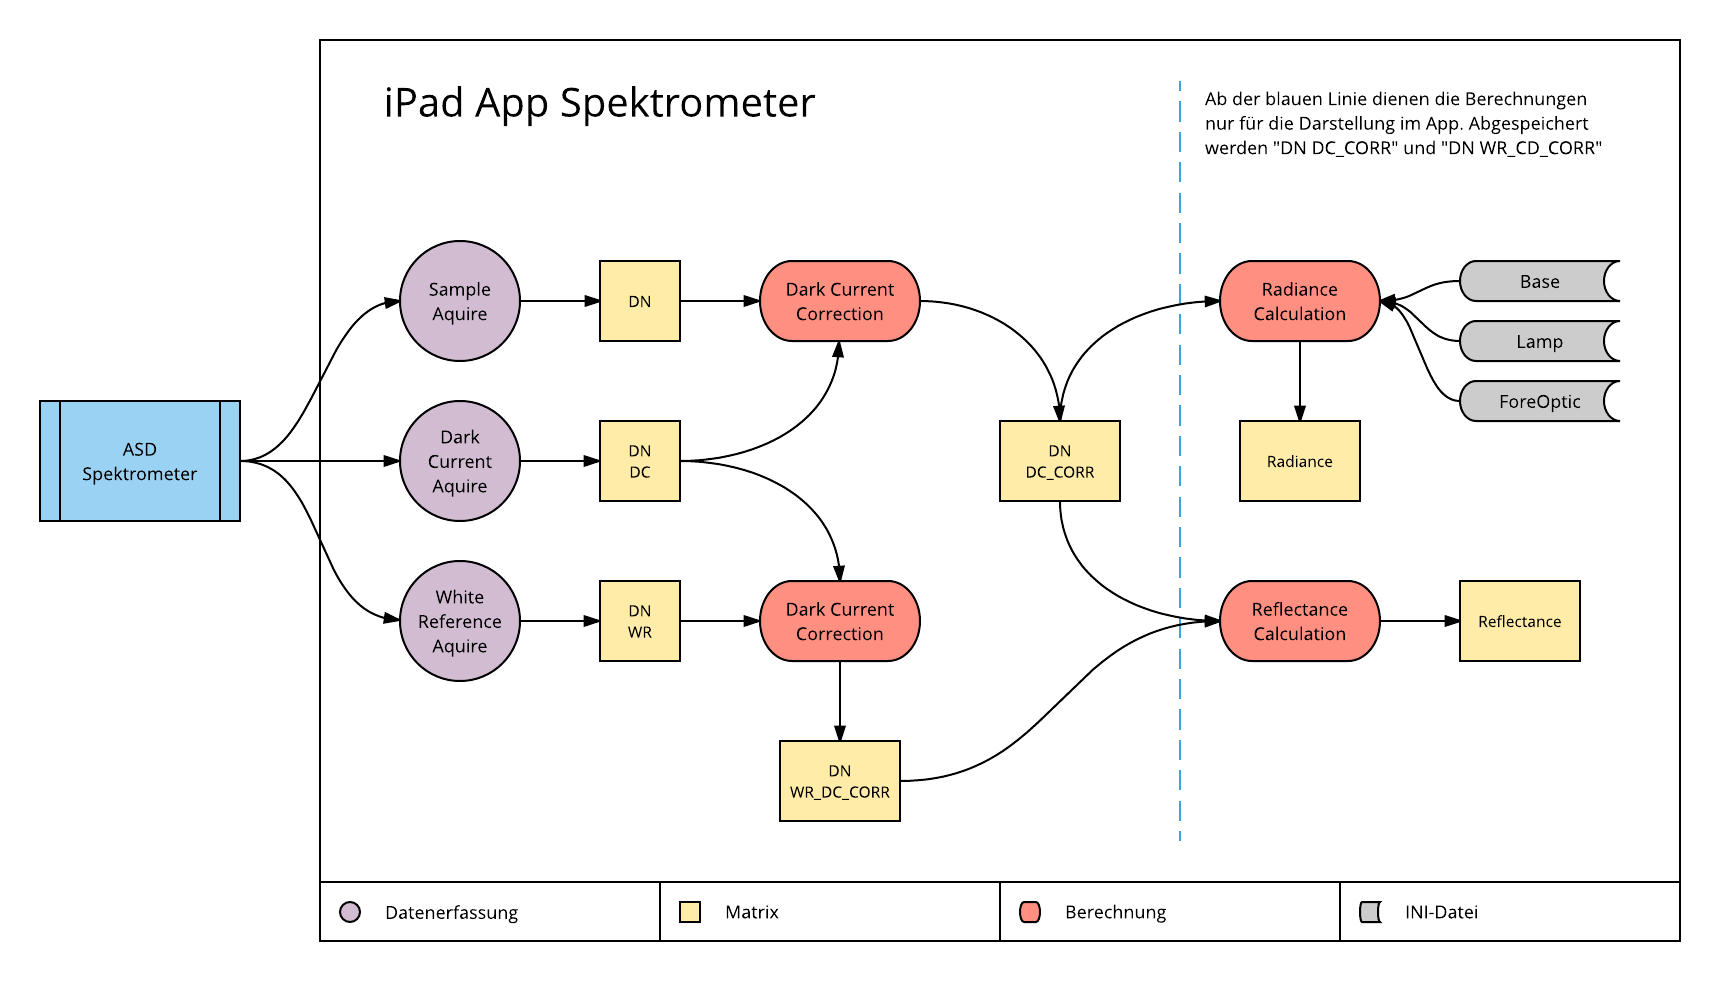
\includegraphics[scale=0.6]{images/Calculations} 
	\caption{Berechnungen f�r Raw, Reflectance und Radiance}
	\label{fig:Calculations}
	\end{center}
\end{figure}

\section{Berechnungen} \label{berechnungen}

\subsection{Dark Current} \label{darkcurrent}

\subsection{White Reference} \label{whitereference}

\subsection{Radiance} \label{radiance}